\begin{figure*}[b]
	\centering
	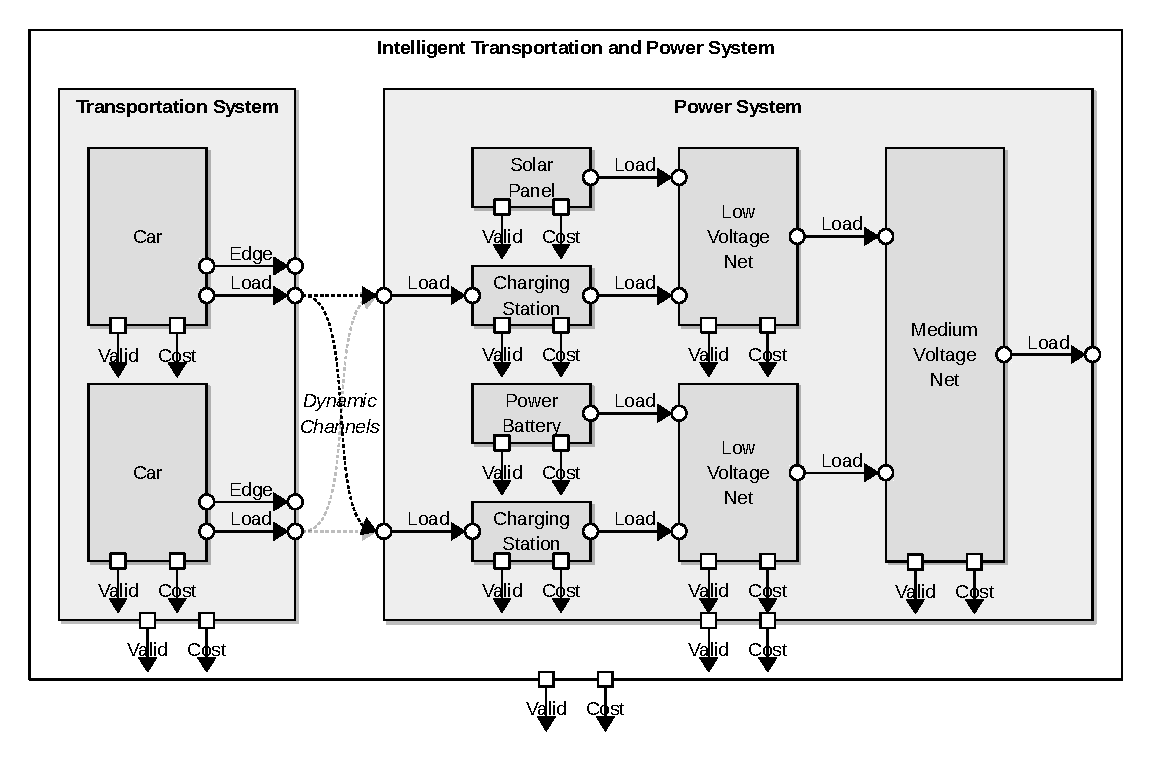
\includegraphics[width=\textwidth]{../gfx/model.pdf}
	\caption{Overview of the holistic modeling approach including transportation and power system connected by dynamic channels.}
	\label{fig:model}
\end{figure*}

\section{Transportation and power system modeling}
\label{section:contribution}

Based on the underlying systems modeling technique (see Section~\ref{section:foundation}), we propose an integrated transportation and power system model as shown in Figure~\ref{fig:model}. At its root, the model defines an intelligent transportation and power system component, which contains separate components for the transportation and the power system. The transportation system component comprises the individual car components traveling along the traffic infrastructure. Similarly, the power system component includes the individual electric components, such as static loads, solar panels, power batteries and charging stations. Furthermore, the power system component contains the electric infrastructure consisting of low-voltage and medium-voltage net components. Parametrization allows one to instantiate all components using reference configurations, i.e. predefined parameter valuations. Subsequently we describe the different components of the model in terms of their parameters, ports, channels and behavior. Furthermore, for each parameter we provide a description as well as a reference configuration.

\subsection{Intelligent transportation and power system ($IS$)}

The intelligent transportation and power system $IS$ component contains the transportation system $TS$ and the power system $PS$ (see following table). Furthermore, the $IS$ defines dynamic channels between the car load outputs of $TS$ and the charging station load inputs of $PS$. Consequently, each car is connected to each charging station statically, but loads are forwarded only to the connected charging station dynamically. Therefore, the dynamic channel conditions test whether the car position (i.e.\ the edge output, see Sec.~\ref{section:car}) matches the charging station position (i.e.\ some constant edge, see Sec.~\ref{section:charging_station}).

\begin{table}[h]
	\renewcommand{\arraystretch}{1.3}
	%\caption{Intelligent transportation and power system parameters}
	\centering
	\begin{tabularx}{\columnwidth}{lllllX}
		\hline
		\textbf{Parameter}      & \textbf{$IS_{A}$} & \textbf{$IS_{B}$}  & \textbf{$IS_{C}$} & \textbf{$IS_{D}$}      & \textbf{Description} \\ \hline
		TS     					& $TS_{A}$   	& $TS_{A}$ & $TS_{A}$ & $TS_{A}$	 	& Transportation system     			\\
		PS               		& $PS_{A}$ 	& $PS_{A}$ & $PS_{B}$ & $PS_{B}$		& Power system   						\\
		w\_TS              & $0.75$  	& $0.25$ & $0.25$ & $0.25$		& Weight of $TS$ cost (\%)	\\ 
		w\_PS              & $0.25$  	& $0.75$ & $0.75$ & $0.75$  		& Weight of $PS$ cost (\%)   			\\ \hline
	\end{tabularx}
\end{table}

Furthermore, the intelligent transportation and power system $IS$ specifies a cost output which aggregates the cost of the transportation system $TS$ and the power system $PS$ using the weights $w\_TS$ and $w\_PS$. On this cost output a minimization objective is defined through annotation. Finally, no additional constraints are defined on system state and behavior.

\subsection{Transportation system ($TS$)}

The transportation system component $TS$ comprises the traffic infrastructure $TN$ as well as the car components $C$ (see following table). The traffic infrastructure $TN$ is modeled as directed graph $G = (V,E)$ with nodes $V$ and edges $E \subseteq V \times V$. Here, nodes $v,w \in V$ represent reference points in the traffic infrastructure such as intersections. Moreover, nodes define an absolute position in real-world coordinates (i.e. latitude, longitude, and elevation). In contrast, edges $(v,w) \in E$ represent road segments between source nodes $v$ and target nodes $w$. Furthermore, edges define their number of lanes as well as their road type (e.g.\ residential streets or stations). The cars $C$, on the other hand, can be configured by means of the parameters $Car\_Number$ and $Car\_Frequency$. While the former defines the total number of cars, the latter models a distribution over available car types. 

\begin{table}[h]
	\renewcommand{\arraystretch}{1.3}
	%\caption{Transportation system parameters}
	\centering
	\begin{tabularx}{\columnwidth}{llX}
		\hline
		\textbf{Parameter}     & \textbf{$TS_{A}$}         & \textbf{Description} \\ \hline
		TN              & $G = (V, E)$    & Traffic network (Graph)    \\
		Car\_Number            & $240$    & Number of $C$s (\#)      \\ 
		Car\_Frequency      & $P(C_{A,B,C}) = 0.\overline{3}$    & Frequency of $C$ types (\%)       \\ \hline
	\end{tabularx}
\end{table}

Finally, the transportation system $TS$ defines a cost output which aggregates the cost of the individual cars $C$. To ensure valid behavior, $TS$ additionally implements a constraint over the car positions which calculates the largest number of pair-wise overlapping cars per segment $(v,w) \in E$ and compares it to the available number of lanes.

\subsection{Car ($C$)}
\label{section:car}

Cars $C$ represent atomic components in our system model and are defined in terms of a range of parameters shown in the following table. Key physical parameters are their $Length$ and $Mass$. Moreover, they contain a battery with predefined state of charge $SOC$. For battery charging and discharging they specify the parameter $Charge\_Rate$.

\begin{table}[h]
	\renewcommand{\arraystretch}{1.3}
	%\caption{Car parameters}
	\centering
	\begin{tabularx}{\columnwidth}{llllX}
		\hline
		\textbf{Parameter}          & \textbf{$C_{A}$} & \textbf{$C_{B}$}  & \textbf{$C_{C}$}           & \textbf{Description} \\ \hline
		Origin                      & $o_A$     & $o_B$ & $o_C$    & Origin position (Edge $E$)      \\
		Destination                 & $d_A$    & $d_B$  & $d_C$     & Destination position (Edge $E$) \\
		Priority                  & $1.0$ & $1.0$ & $1.0$ & Priority of the car in traffic (\%)                  \\
		Length                    & $4.0$ & $4.0$ & $4.0$ & Car length (Meters)            \\
		Mass                   & $2.0$ & $2.0$ & $2.0$ & Car mass  (Tonnes)                 \\
		Energy\_Economy				& $0.4$ & $0.4$ & $0.4$ & Energy consumption (kW/h/km) \\
		Speed\_Max				& $50.0$ & $50.0$ & $50.0$ & Max. driving speed (km/h) \\
		SOC                      & $30.0$ & $60.0$ & $90.0$ & Initial state of charge (kW/h)                   \\
		SOC\_Min               & $0.0$ & $0.0$ & $0.0$ & Min. state of charge (kW/h)                     \\
		SOC\_Max              & $90.0$ & $90.0$ & $90.0$ & Max. state of charge (kW/h)                      \\
		Charge\_Rate          & $5.0$ & $5.0$ & $5.0$ & Battery (dis-)charge rate (kW/h)                    \\
		Range\_Anxiety         & $0.2$ & $0.2$ & $0.2$ & Affinity to charge (\%)                     \\
		CS\_Selection		   & $0.5$ & $0.5$ & $0.5$ & Charging station randomness (\%)                    \\ 
		Departure\_Time 	& $0$ & $0$ & $0$ & Offset to start traveling (Minutes)                   \\
		w\_SOC              & $0.\overline{3}$  & $0.\overline{3}$ & $0.\overline{3}$ & Weight of state of charge cost (\%)                   \\
		w\_Time              & $0.\overline{3}$ & $0.\overline{3}$ & $0.\overline{3}$ & Weight of time cost (\%)                     \\
		w\_Power             & $0.\overline{3}$ & $0.\overline{3}$ & $0.\overline{3}$ & Weight of power cost (\%)                      \\ \hline
	\end{tabularx}
\end{table}

During simulation, when the time point $Departure\_Time$ is passed the car starts traveling from origin $Origin$ to destination $Destination$. Origins, destinations and current position of cars are edges $v \in V$ of the traffic infrastructure $TN$. When starting to travel, the car position equals the origin, while subsequent positions are selected from a set of possible routes. The set of possible routes equals to the $k \in \mathbb{N}$ shortest paths from the current position to the destination or the nearest charging station. Of these alternatives one route is selected randomly depending on the parameter $CS\_Selection$. If the state of charge falls below a specified percentage described by the parameter $Range\_Anxiety$, the route selection probability shifts towards preferring the nearest charging station. While driving along the traffic infrastructure, cars consume energy. The energy consumption is based on the energy economy parameter $Energy\_Economy$, the traveled elevation profile, the mass as well as the randomly selected speed. Hereby, the speed is limited by the parameter $Speed\_Max$. Both energy consumption and possibly production are applied to the state of charge. Consumption occurs during driving or during discharge at charging stations. Production occurs during driving (i.e.\ energy recuperation) or during charging at charging stations instead. To ensure valid behavior, a constraint tests whether the state of charge lies within a constant minimum $SOC\_Min$ and maximum $SOC\_Max$. When connected to a charging station, the (dis-)charging decision is taken randomly with uniform distribution. If the car charges, a predefined load is transferred from the charging station to the car. If the car discharges, a predefined load (i.e.\ charge rate) is transferred from the car to the charging station instead. Furthermore, the car can choose an idle state, in which case no load is transferred between car and charging station. Finally, the car objective includes multiple cost factors. Generally, car cost only accumulate after its departure time $Departure\_Time$ has passed. The fist cost factor evaluates the car's state of charge with respect to the car's maximum state of charge. The second cost factor aggregates the time needed to reach the destination $Destination$. And the third cost factor measures the energy consumption in relation to the maximum energy consumption. The cost factors are aggregated and weighted using the parameters $w\_SOC$, $w\_Time$ and $w\_Power$.

\subsection{Power system ($PS$)}

The power system component $PS$ represents the overall electric infrastructure including individual electric devices as well as low-voltage nets $LV$ and medium-voltage nets $MV$ (higher voltage nets are omitted currently). Currently supported devices include static loads $SL$, solar panels $SP$, power batteries $PB$ and charging stations $CS$. Furthermore, the power system can be configured using a number of parameters which are summarized in the following table.

\begin{table}[h]
	\renewcommand{\arraystretch}{1.3}
	%\caption{Power system parameters}
	\centering
	\begin{tabularx}{\columnwidth}{lllX}
		\hline
		\textbf{Parameter}     & \textbf{$PS_{A}$} & \textbf{$PS_{B}$}       & \textbf{Description} \\ \hline
		TN              	   & $G=(E,V)$ & $G=(E,V)$    	  & Traffic network (Graph)     \\
		LV\_Number             & $4$ & $4$            & Number of $LV$s (\#)      \\
		LV\_Frequency          & $P(LV_{A})=1$ & $P(LV_{A})=1$                & Freq. of $LV$ types (\%)      \\
		LV\_Allocation         & $9$ & $19$                 & Elec.\ dev.\ per $LV$ (\#)      \\   
		MV\_Number             & $1$ & $1$        & Number of $MV$s (\#)      \\ 
		MV\_Frequency          & $P(MV_{A})=1$ & $P(MV_{A})=1$                & Freq.\ of $MV$ types (\%)      \\
		MV\_Allocation         & $4$ & $4$                     & $LV$s per $MV$ (\#)      \\   
		SL\_Number             & $10$ & $10$              & Number of $SL$s (\#)      \\
		SL\_Frequency          & $P(SL_{A})=1$ & $P(SL_{B})=1$              & Freq.\ of $SL$ types (\%)       \\
		SP\_Number             & $5$ & $5$         & Number of $SP$s (\#)      \\ 
		SP\_Frequency          & $P(SP_{A})=1$ & $P(SP_{B})=1$                & Freq.\ of $SP$ types (\%)       \\  
		CS\_Number             & $16$  & $56$           & Number of $CS$s (\#)      \\
		CS\_Frequency          & $P(CS_{A})=1$  & $P(CS_{B})=1$               & Freq.\ of $CS$ types (\%)       \\   
		PB\_Number             & $5$  & $5$              & Number of $PB$s (\#)      \\
		PB\_Frequency          & $P(PB_{A})=1$ & $P(PB_{B})=1$              & Freq.\ of $PB$ types (\%)       \\   \hline  
	\end{tabularx}
\end{table}

At its interface the power system specifies a cost output that aggregates the cost of the power batteries $PB$, solar panels $SP$, charging stations $CS$ as well as low- and medium-voltage networks $LV$/$MV$. In principle, different aggregation schemes can be used. Furthermore, it forwards the load of the medium-voltage network representing the final load balance.

\subsection{Low/medium-voltage nets ($LV$/$MV$)}

Low- and medium-voltage nets $LV$, $MV$ represent one part of the electric infrastructure. In our model, low- and medium-voltage nets receive the loads of all connected electric devices and provide an aggregate load to the upper voltage level.

\begin{table}[h]
	\renewcommand{\arraystretch}{1.3}
	%\caption{Low/medium voltage net parameters}
	\centering
	\begin{tabularx}{\columnwidth}{lllX}
		\hline
		\textbf{Parameter}   & \textbf{$LV_{A}$} & \textbf{$MV_{A}$}  & Description \\ \hline
		w\_Balance       & $0.0$ & $1.0$ & Weight of balance costs (\%) \\  
%		Size                  	  & $9$ & $19$ & Number of devices per net  (\#)    \\
		Capacity          & $20.0$ & $200.0$ & Power load capacity (kW/h)     \\ \hline
	\end{tabularx}
\end{table}

In terms of behavior, the low-voltage net aggregates the loads of all connected static load, power batteries, solar panels, charging stations to a single power load. The medium voltage net aggregates the power loads of low voltage nets it is assigned to a single power load. Based on this aggregation, a cost function over the total power load balance is specified. The cost function is multiplied by the impact of the balance objective through an according weight, specified by parameter $w\_Balance$. To ensure valid behavior, a constraint tests whether the net's total power load balance lies within the net' total capacity, described by parameter $Capacity$.

\subsection{Static load ($SL$)}

Static loads $SL$ are aggregations of energy devices, which produce intermittent energy load balances. They represent an abstraction in terms of aggregating power loads of different energy devices, i.e. producers and consumers. The result of this aggregation is a energy load profile $P = (T, L)$ describing the energy load $L$ over time $T$ for values $L = \{l_i, l_{i+1}, ..., l_n\}$ and $T = \{t_i, t_{i+1},..., t_n\}$.

\begin{table}[h]
	\renewcommand{\arraystretch}{1.3}
	%\caption{Static load parameters}
	\centering
	\begin{tabularx}{\columnwidth}{lllX}
		\hline
		\textbf{Parameter}              & \textbf{$SL_{A}$}  & \textbf{$SL_{B}$}   & \textbf{Description} \\ \hline
		Power\_Scale                   	  & $10.0$ & $5.0$ & Maximum power output (kW/h) \\
		Profile                       	  	   & $P_A$ & $P_B$ & Load profile over time  (kW/h)\\ \hline
	\end{tabularx}
\end{table}

In their behavior, based on the parameters $Power\_Scale$ and $Profile$ static load components produce a predefined energy profile for a given time. Both parameters allow one to vary static (i.e.\ non-controllable) load in different scenarios easily.

\subsection{Power battery ($PB$)}

Power batteries $PB$ represent electric devices which act as energy producers or energy consumers within the electric network.
This is key to their ability to store or release energy over time.

\begin{table}[h]
	\renewcommand{\arraystretch}{1.3}
	%\caption{Power battery parameters}
	\centering
	\begin{tabularx}{\columnwidth}{lllX}
		\hline
		\textbf{Parameter}     & \textbf{$PB_{A}$} & \textbf{$PB_{B}$} & \textbf{Description} \\ \hline
		SOC                     & $0.0$ & $0.0$ & Initial state of charge (kW/h)                   \\
		SOC\_Min                & $0.0$ & $0.0$ & Min. state of charge (kW/h)                   \\
		SOC\_Max               & $20.0$ & $80.0$ &  Max. state of charge (kW/h)                    \\
		Charge\_Rate            & $5.0$ & $5.0$ & Battery (dis-)charge rate (kW/h)     \\ 
		Battery\_Loss           & $0.05$ & $0.05$ & Loss of charge over time (\%)\\
		Battery\_Efficiency      & $0.99$ & $0.99$ &Efficiency of (dis-)charging (\%)     \\ \hline
	\end{tabularx}
\end{table}

In terms of behavior, based on probabilistic selection, the power battery chooses from different states determining energy consumption, production or zero load. In terms of probability, states are uniformly distributed. Energy consumption or production occurs by storing or releasing energy based the state of charge, which is initially specified by parameter $SOC$. This ability is subject to loss of charge over time and to the battery's efficiency, respectively described by parameters $Battery\_Loss$ and $Battery\_Efficiency$.
Energy consumption occurs by storing energy in the battery, while energy production occurs by releasing energy from the battery. Both actions are subject to a limited charge and discharge rate, specified by parameter $Charge\_Rate$. To ensure valid behavior, a constraint tests whether the battery's state of charge lies within a constant minimum and maximum level expressed through parameters $SOC\_Min$ and $SOC\_Max$.

\subsection{Solar panel ($SP$)}

Solar panels $SP$ are electric devices, which act as producers of renewable energy with a defined yield within the electric network. They are characterized by their situation related power production capabilities. 

\begin{table}[h]
	\renewcommand{\arraystretch}{1.3}
	%\caption{Solar panel parameters}
	\centering
	\begin{tabularx}{\columnwidth}{lllX}
		\hline
		\textbf{Parameter}                     & \textbf{$SP_{A}$} & \textbf{$SP_{B}$} & \textbf{Description} \\ \hline
		Power\_Scale                       	   & $2.5$ & $10.0$ & Maximum power output (kW/h) \\
		Mean                       	  		  & $15$ & $15$ & Mean for maximum power output (\#) \\
		Variance                       	       & $5$ & $5$ & Variance for maximum power output (\#) \\ \hline
	\end{tabularx}
\end{table}

In terms of behavior, based on it's specific power scale, the solar panel produces an power load determined by given mean of and variance of maximum power output within a given time, respectively described by parameters $Power\_Scale$, $Mean$ and $Variance$. Based on a probabilistic selection, the solar panel can choose to partially, fully or not dampen it's power load, representing a property of a smart energy producer. The probability of these options is uniformly distributed.

\subsection{Charging station ($CS$)}
\label{section:charging_station}

Charging stations $CS$ are electric devices which act as power consumers or producers within the electric network and facilitate the charging process of the cars of the transportation system. They are assigned a physical location, i.e. specific position on the traffic network. 

\begin{table}[h]
	\renewcommand{\arraystretch}{1.3}
	%\caption{Charging station parameters}
	\centering
	\begin{tabularx}{\columnwidth}{llX}
		\hline
		\textbf{Parameter}      & \textbf{$CS_{A}$} & \textbf{Description} \\ \hline
		Position      			& $E$ & Position on the traffic network (Edge $E$) \\  
		Charge\_Rate        	& $5.0$ & (Dis-)charge rate exposed to cars (kW/h)     \\ \hline
	\end{tabularx}
\end{table}

In terms of their behavior, charging stations can exhibit zero, negative or positive power load. Based on connection to a car, the charging station's behavior is determined by the selected charging state of the connected car being located at the charging stations position, specified by parameter $Position$. They act as energy consumers, when a power load is transferred from the charging station to the connected car. Furthermore, they act as energy producers, when a power load is transferred from the connected car to the charging station. The rate to which power loads can be transferred is described as parameter $Charge\_Rate$.